% Introduction chapter.
%%%%%%%%%%%%%%%%%%%%%%%

\chapter{Introduction}

The program relax is designed for the study of the dynamics of proteins or other macromolecules though the analysis of NMR relaxation data.  It is a community driven project created by NMR spectroscopists for NMR spectroscopists.  It supports exponential curve fitting for the calculation of the $\Rone$ and $\Rtwo$ relaxation rates, calculation of the NOE, reduced spectral density mapping, and the Lipari and Szabo model-free analysis.


The aim of relax is to provide a seamless and extremely flexible environment able to accept input in any format produced by other NMR software, able to faultlessly create input files, control, and read output from various programs including Modelfree and Dasha, output results in many formats, and visualise the data by controlling programs such as Grace\index{software!Grace|textbf}, OpenDX\index{software!OpenDX|textbf}, MOLMOL\index{software!MOLMOL|textbf}, and PyMOL\index{software!PyMOL|textbf}.  All data analysis tools from optimisation to model selection to Monte Carlo simulations are inbuilt into relax. Therefore the use of additional programs is optional.

The flexibility of relax arises from the choice of either relax's scripting capabilities or its Python\index{Python|textbf} prompt interface. Extremely complex scripts can be created from simple building blocks to fully automate data analysis. A number of sample scripts have been provided to help understand script construction. In addition, any of Python's powerful features or functions can be incorporated as the script is executed as an arbitrary Python source file within relax's environment.  The modules of relax can also used as a vast library of dynamics related functions by your own software.

relax is free software (free as in freedom) which is licenced under the GNU General Public Licence (GPL)\index{GPL|textbf}. You are free to copy, modify, or redistribute relax under the terms of the GPL. 


% Program features.
%%%%%%%%%%%%%%%%%%%

\section{Program features}


% Literature.
%~~~~~~~~~~~~

\subsection{Literature}

The primary references for the program relax are \citet{dAuvergneGooley08a} and \citet{dAuvergneGooley08b}.

Other literature related to the improved model-free analysis used within relax, which can nevertheless be applied to other techniques such as SRLS\index{SRLS}, include model-free model selection \citep{dAuvergneGooley03, Chen04}\index{model selection}, model-free model elimination \citep{dAuvergneGooley06}\index{model elimination}, the theory \citep{dAuvergneGooley07} behind the new model-free optimisation protocol \citep{dAuvergneGooley08b}, and the hybridisation of different models \citep{Horne07, dAuvergneGooley08b}. Most of these details can be found in the PhD thesis of \citet{dAuvergne06}.


% Supported NMR theories.
%~~~~~~~~~~~~~~~~~~~~~~~~

\subsection{Supported NMR theories}

The following relaxation data analysis techniques are currently supported by relax:

\begin{itemize}
\item Model-free analysis \citep{LipariSzabo82a, LipariSzabo82b, Clore90a}.
\item Reduced spectral density mapping \citep{Farrow95, Lefevre96}\index{reduced spectral density mapping}.
\item Exponential curve fitting (to find the $\Rone$ and $\Rtwo$ relaxation rates)\index{exponential curve fitting}.
\item Steady-state NOE calculation\index{NOE}.
\end{itemize}


% The future.
\subsubsection{The future}

At some time in the future the following techniques are planned to be implemented within relax:

\begin{itemize}
\item Relaxation dispersion\index{relaxation dispersion}.
\item SRLS -- Slowly relaxing local structure \citep{Tugarinov01}\index{SRLS}.
\end{itemize}

Because relax is free software, if you would like to contribute addition features, functions, or modules which you have written for your own publications for the benefit of the field, almost anything relating to molecular dynamics may be accepted.  Please see the Open Source chapter for more details.



% Data analysis tools.
%~~~~~~~~~~~~~~~~~~~~~

\subsection{Data analysis tools}

The following tools are implemented as modular components to be used by any data analysis technique:

\begin{itemize}
\item Numerous high-precision optimisation algorithms\index{minisation}.
\item Model selection \citep{dAuvergneGooley03, Chen04}\index{model selection}:
    \begin{itemize}
    \item Akaike's Information Criteria (AIC)\index{model selection!AIC}.
    \item Small sample size corrected AIC (AICc)\index{model selection!AICc}.
    \item Bayesian or Schwarz Information Criteria (BIC)\index{model selection!BIC}.
    \item Bootstrap model selection\index{model selection!bootstrap}.
    \item Single-item-out cross-validation (CV)\index{model selection!cross-validation}.
    \item Hypothesis testing ANOVA model selection (only the model-free specific technique of \citet{Mandel95} is supported)\index{model selection!hypothesis testing}\index{model selection!ANOVA}.
    \end{itemize}
\item Monte Carlo simulations (error analysis for all data analysis techniques)\index{Monte Carlo simulation}.
\item Model elimination -- the removal of failed models prior to model selection \citep{dAuvergneGooley06}\index{model elimination}.
\end{itemize}


% Data visualisation.
%~~~~~~~~~~~~~~~~~~~~

\subsection{Data visualisation}

The results of an analysis, or any data input into relax, can be visualised using a number of programs:

\begin{description}
\item[MOLMOL] 1D data can be mapped onto a structure either by the creation of MOLMOL macros or by direct control of the program\index{software!MOLMOL}.
\item[PyMOL] 3D objects such as the diffusion tensor representation can be displayed with the structure\index{software!PyMOL}.
\item[Grace] any 2D data can be plotted\index{software!Grace}.
\item[OpenDX] The chi-squared space of models with three parameters can be mapped and 3D images of the space produced\index{software!OpenDX}.
\end{description}


% Interfacing with other programs.
%~~~~~~~~~~~~~~~~~~~~~~~~~~~~~~~~~

\subsection{Interfacing with other programs}

relax can create the input files, execute in-line, and then read the output of the following programs. These programs can be used as optimisation engines replacing the minimisation algorithms built into relax:

\begin{itemize}
\item Dasha (model-free analysis)\index{software!Dasha}.
\item Modelfree (model-free analysis)\index{software!Modelfree}.
\end{itemize}


% The user interfaces (UI).
%~~~~~~~~~~~~~~~~~~~~~~~~~~

\subsection{The user interfaces (UI)}

relax can be used through the following UIs:

\begin{description}
\item[The prompt] this is the primary interface of relax. Rather than reinventing a new command language, relax's interface is the powerful Python prompt. This gives the power user full access to a proven programming language.
\item[Scripting] this provides a more powerful and flexible framework for controlling the program. The script will be executed as Python code enabling advanced programming for automating data analysis. All the features available within the prompt environment are accessible to the script.
\item[GUI] the graphical user interface provides a sub-set of relax's features - the automatic R$_1$ and R$_2$ relaxation rate curve-fitting, the NOE calculations, and the automatic model-free analysis provided by the dauvergne\_protocol module \citep{dAuvergneGooley08b}.
\end{description}



% The relax HOWTO.
%%%%%%%%%%%%%%%%%%

\section{How to use relax}


% The prompt.
%~~~~~~~~~~~~

\subsection{The prompt}
\index{prompt|textbf}

% Prompt screenshot
\begin{figure}
\centerline{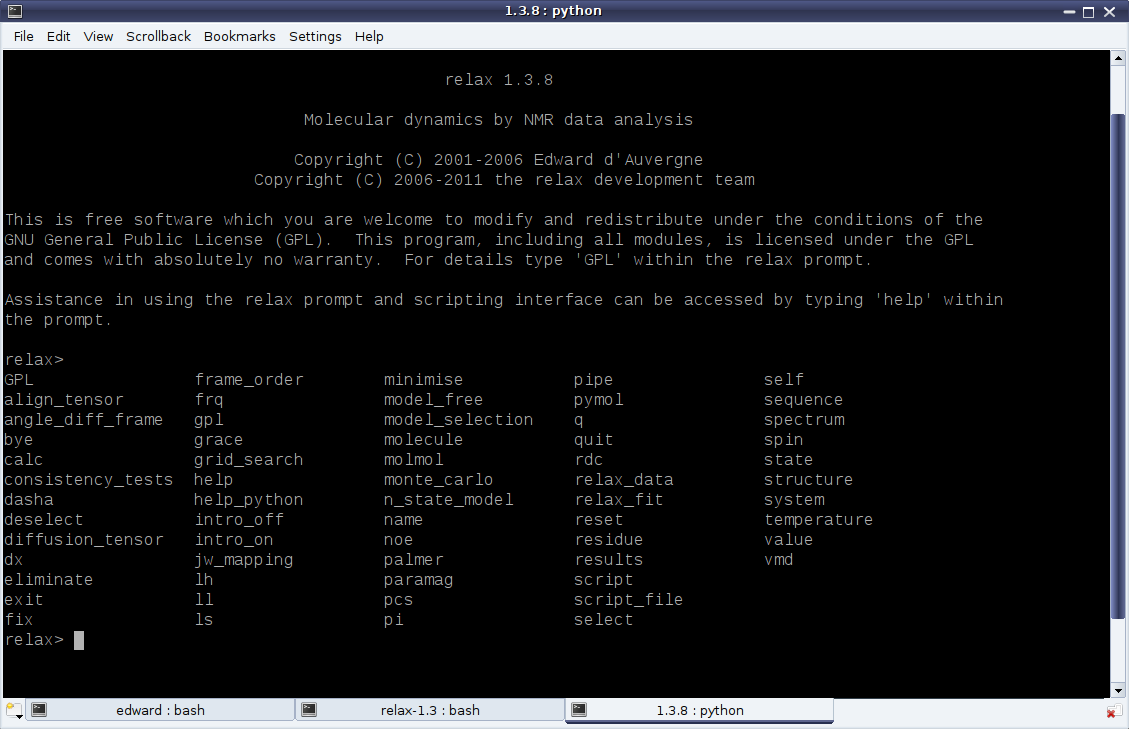
\includegraphics[width=\textwidth, bb=0 0 1122 729]{graphics/screenshots/relax_prompt_1_3_8.png}}
\caption[Prompt screenshot]{A screenshot of relax being run in the primary prompt mode.}\label{fig: relax prompt}
\end{figure}

The primary interface of relax is the prompt.  After typing \texttt{`relax'} within a terminal\index{terminal} you will be presented with

\example{relax>}

This is the Python prompt which has been tailored specifically for relax.  You will hence have full access, if desired, to the power of the Python\index{Python} programing language to manipulate your data.  You can for instance type

\example{relax> print "Hello World"}

the result being

\begin{exampleenv}
relax> print "Hello World" \\
Hello World \\
relax>
\end{exampleenv}

Or using relax as a calculator

\begin{exampleenv}
relax> (1.0 + (2 * 3))/10 \\
0.69999999999999996 \\
relax>
\end{exampleenv}



% Python.
%~~~~~~~~

\subsection{Python}

\index{Python|textbf}
relax has been designed such that knowledge about Python is not required to be able to fully use the program.  A few basics though will aid in understanding relax.

A number of simple programming axioms includes that of strings\index{string}, integers\index{integer}, floating point numbers\index{floating point number}, and lists\index{list}.  A string is text and within Python (as well as relax) this is delimited by either single or double quotes.  An integer is a number with no decimal point whereas a float is a number with a decimal point.  A list in Python (called an array in other languages) is a list of anything separated by commas and delimited by square brackets, an example is [0, 1, 2, `a', 1.2143235].

Probably the most important detail is that functions in Python require brackets around their arguments.  For example

\example{relax> minimise()}

will commence minimisation\index{minimisation} however

\example{relax> minimise}

will do nothing.

The arguments to a function are simply a comma separated list within the brackets of the function.  For example to save the program's current state type

\example{relax> state.save(`save', force=True)}

Two types of arguments exist in Python\index{Python|textbf} -- standard arguments\index{argument} and keyword arguments\index{keyword argument}\index{argument!keyword}.  The majority of arguments you will encounter within relax are keyword arguments however you may, in rare cases, encounter a non-keyword argument.  For these standard arguments just type the values in, although they must be in the correct order.  Keyword arguments consist of two parts -- the key and the value.  For example the key may be \texttt{file} and the value you would like to supply is \texttt{`R1.out'}.  Various methods exist for supplying this argument.  Firstly you could simply type \texttt{`R1.out'} into the correct position in the argument list.  Secondly you can type \texttt{file=`R1.out'}.  The power of this second option is that argument order is unimportant.  Therefore if you would like to change the default value of the very last argument, you don't have to supply values for all other arguments.  The only catch is that standard arguments must come before the keyword arguments.



% User functions.
%~~~~~~~~~~~~~~~~

\subsection{User functions}
\index{user functions|textbf}

For standard data analysis a large number of specially tailored functions called `user functions' have been implemented.  These are accessible from the relax prompt by simply typing the name of the function.  An example is \texttt{`help()'}\index{help system}.  An alphabetical listing of all accessible user functions together with full descriptions is presented later in this manual.

A few special objects which are available within the prompt are not actually functions.  These objects do not require brackets at their end for them to function.  For example to exit relax type

\example{relax> exit}

Another special object is that of the function class\index{function class}.  This object is simply a container which holds a number of user functions.  You can access the user function within the class by typing the name of the class, then a dot \texttt{`.'}, followed by the name of the user function.  An example is the user function for reading relaxation data out of a file and loading the data into relax.  The function is called \texttt{`read'} and the class is called \texttt{`relax\_data'}.  To execute the function, type something like

\example{relax> relax\_data.read(`R1', `600', 600.0 * 1e6, `r1.600.out')}

On first usage the relax prompt can be quite daunting.  Two features exist to increase the usability of the prompt -- the help system and tab completion.



% The help system.
%~~~~~~~~~~~~~~~~~

\subsection{The help system}
\index{help system|textbf}

For assistance in using a function simply type

\example{help(function)}

In addition to functions if

\example{help(object)}

is typed the help for the python object is returned.  This system is similar to the help function built into the python interpreter, which has been renamed to \texttt{help\_python}, with the interactive component removed.  For the standard interactive python help system type

\example{help\_python()}




% Tab completion.
%~~~~~~~~~~~~~~~~

\subsection{Tab completion}
\index{tab completion|textbf}

Tab completion is implemented to prevent insanity as the function names can be quite long -- a deliberate feature to improve usability.  The behaviour of the tab completion is very similar to that of the bash prompt.

Not only is tab completion useful for preventing RSI but it can also be used for listing all available functions.  To begin with if you hit the [TAB] key without typing any text all available functions will be listed (along with function classes\index{function class} and other python objects).  This extends to the exploration of user functions\index{user functions} within a function class\index{function class}.  For example to list the user functions within the function class \texttt{`model\_free'} type

\example{relax> model\_free.}

The dot character at the end is essential.  After hitting the [TAB] key you should see something like

\begin{exampleenv}
relax> model\_free. \\
model\_free.\_\_class\_\_ \\
model\_free.\_\_doc\_\_ \\
model\_free.\_\_init\_\_ \\
model\_free.\_\_module\_\_ \\
model\_free.\_\_relax\_\_ \\
model\_free.\_\_relax\_help\_\_ \\
model\_free.create\_model \\
model\_free.delete \\
model\_free.remove\_tm \\
model\_free.select\_model \\
relax> model\_free.
\end{exampleenv}

All the objects beginning with an underscore are ``hidden'', they contain information about the function class\index{function class} and should be ignored.  From the listing the user functions\index{user functions} \texttt{`copy'}, \texttt{`create\_model'}, \texttt{`delete'}, \texttt{`remove\_tm'}, and \texttt{`select\_model'} contained within \texttt{`model\_free'} are all visible.



% The data pipe.
%~~~~~~~~~~~~~~~

\subsection{The data pipe}
\index{data pipe|textbf}

Within relax all user functions operate on data stored within the current data pipe.  This pipe stores data is input, processed, or output as user functions are called.  There are different types of data pipe for different analyses, e.g. a reduced spectral density mapping pipe, a model-free pipe, an exponential curve-fitting pipe, etc.  Multiple data pipes can be created within relax and various operations performed in sequence on these pipes.  This is useful for operations such as model selection whereby the function \texttt{`model\_selection'} can operate on a number of pipes corresponding to different models and then assign the results to a newly created pipe.  When running relax you choose which pipe you are currently in by using the \texttt{`pipe.switch'} user function to jump between pipes. 

The flow of data through relax can be thought of as travelling through these pipes.  User functions\index{user functions} exist to transfer data between these pipes and other functions combine data from multiple pipes into one or vice versa.  The simplest invocation of relax would be the creation of a single data pipe and with the data being processed as it is passing through this pipe.

The primary method for creating a data pipe is through the user function\index{user functions} \texttt{`pipe.create'}.  For example

\example{relax> pipe.create(`m1', `mf')}

will create a model-free data pipe labelled \texttt{`m1'}.  The following is a table of all the types which can be assigned to a data pipe.

\begin{center}
\begin{tabular}{ll}
\toprule

Data pipe type          & Description \\

\midrule

\texttt{`jw'}           & Reduced spectral density mapping \\
\texttt{`mf'}           & Model-free data analysis \\
\texttt{`N-state'}      & N-state model of domain motions \\
\texttt{`noe'}          & Steady state NOE calculation \\
\texttt{`relax\_fit'}   & Relaxation curve-fitting \\
\texttt{`srls'}         & SRLS analysis \\

\bottomrule
\end{tabular}
\end{center}

Currently the NOE calculation, relaxation curve-fitting, model-free analysis, and reduced spectral density mapping features of relax are implemented (if this documentation is out of date then you may be able to do a lot more).



% Scripting.
%~~~~~~~~~~~

\subsection{Scripting}
\index{scripting|textbf}

What ever is done within the prompt is also accessible through scripting.  Just type your commands into a text file and then at the terminal type

\example{\$ relax your\_script}

An example of a simple script which will minimise the model-free model `m4' after loading six relaxation data sets is

\begin{exampleenv}
\# Create the data pipe. \\
name = `m4' \\
pipe.create(name, `mf') \\
 \\
\# Nuclei type \\
nuclei(`N') \\
 \\
\# Load the sequence. \\
sequence.read(`noe.500.out') \\
 \\
\# Load the relaxation data. \\
relax\_data.read(`R1', `600', 600.0 * 1e6, `r1.600.out') \\
relax\_data.read(`R2', `600', 600.0 * 1e6, `r2.600.out') \\
relax\_data.read(`NOE', `600', 600.0 * 1e6, `noe.600.out') \\
relax\_data.read(`R1', `500', 500.0 * 1e6, `r1.500.out') \\
relax\_data.read(`R2', `500', 500.0 * 1e6, `r2.500.out') \\
relax\_data.read(`NOE', `500', 500.0 * 1e6, `noe.500.out') \\
 \\
\# Setup other values. \\
diffusion\_tensor.init((2e-8, 1.3, 60, 290), param\_types=1, axial\_type=`prolate', fixed=True) \\
value.set(1.02 * 1e-10, `bond\_length') \\
value.set(-160 * 1e-6, `csa') \\
value.set(`15N', `heteronucleus') \\
value.set(`1H', `proton') \\
 \\
\# Select a preset model-free model. \\
model\_free.select\_model(model=name) \\
 \\
\# Grid search. \\
grid\_search(inc=11) \\
 \\
\# Minimise. \\
minimise(`newton') \\
 \\
\# Finish. \\
results.write(file=`results', force=True) \\
state.save(`save', force=True)
\end{exampleenv}

Scripting is much more powerful than the prompt as advanced Python\index{Python} programming can be employed (see the file `full\_analysis.py' in the `sample\_scripts' directory for an example).



% Sample scripts.
%~~~~~~~~~~~~~~~~

\subsection{Sample scripts}
\index{scripting!sample scripts}

A few sample scripts have been provided in the directory `sample\_scripts'.  These can be copied and modified for different types of data analysis.



% The test suite.
%~~~~~~~~~~~~~~~~

\subsection{The test suite}
\index{test suite}

To test that the program functions correctly, relax possesses an inbuilt test suite.  The suite is a collection of simple tests which execute or probe different parts of the program checking that the software runs without problem.  The test suite is executed by running relax using the command \texttt{`relax --test-suite'}.



% The GUI.
%~~~~~~~~~

\subsection{The GUI}
\index{GUI}

relax has been designed primarily for scripting and, as such, no graphical user interface (GUI) currently exists.  The internal structure of the program has been specifically designed so any type of control mechanism can be easily added, including a GUI, therefore in the future one may be written.  A GUI will, however, detract from the power and flexibility inherent in the control by scripting.



% Access to the internals of relax.
%~~~~~~~~~~~~~~~~~~~~~~~~~~~~~~~~~~

\subsection{Access to the internals of relax}

To enable advanced Python\index{Python} scripting and control many parts of relax have been designed in an object oriented fashion.  If you would like to play with internals of the program the entirety of relax is accessible by importation.  For example all data is contained within the object called the relax data store which, to be able to access it, needs be imported by typing:

\example{relax> from data import Data as relax\_data\_store}

This is a dictionary type object which contains the multiple data pipes.  All of relax's packages, modules, functions, and classes are also accessible by import statements.  For example to create a rotation matrix from three Euler angles in the z-y-z notation, type:

\begin{exampleenv}
relax> alpha = 0.1342 \\
relax> beta = 1.0134 \\
relax> gamma = 2.4747 \\
relax> from maths\_fns.rotation\_matrix import R\_euler\_zyz \\
relax> from numpy import float64, zeros \\
relax> R = zeros((3,3), float64) \\
relax> R\_euler\_zyz(R, alpha, beta, gamma) \\
relax> R
\end{exampleenv}



% Usage of the name relax.
%~~~~~~~~~~~~~~~~~~~~~~~~~

\section{Usage of the name relax}

The program relax is so relaxed that the first letter should always be in lower case!
